
\begin{frame}{Panel Factorization}
\framesubtitle{Comparative study}
\begin{itemize}
\item Natural Version
\item Implemented Version
\end{itemize}
\end{frame}

\begin{frame}{Panel Factorization}
\framesubtitle{Panel operations}
\begin{center}
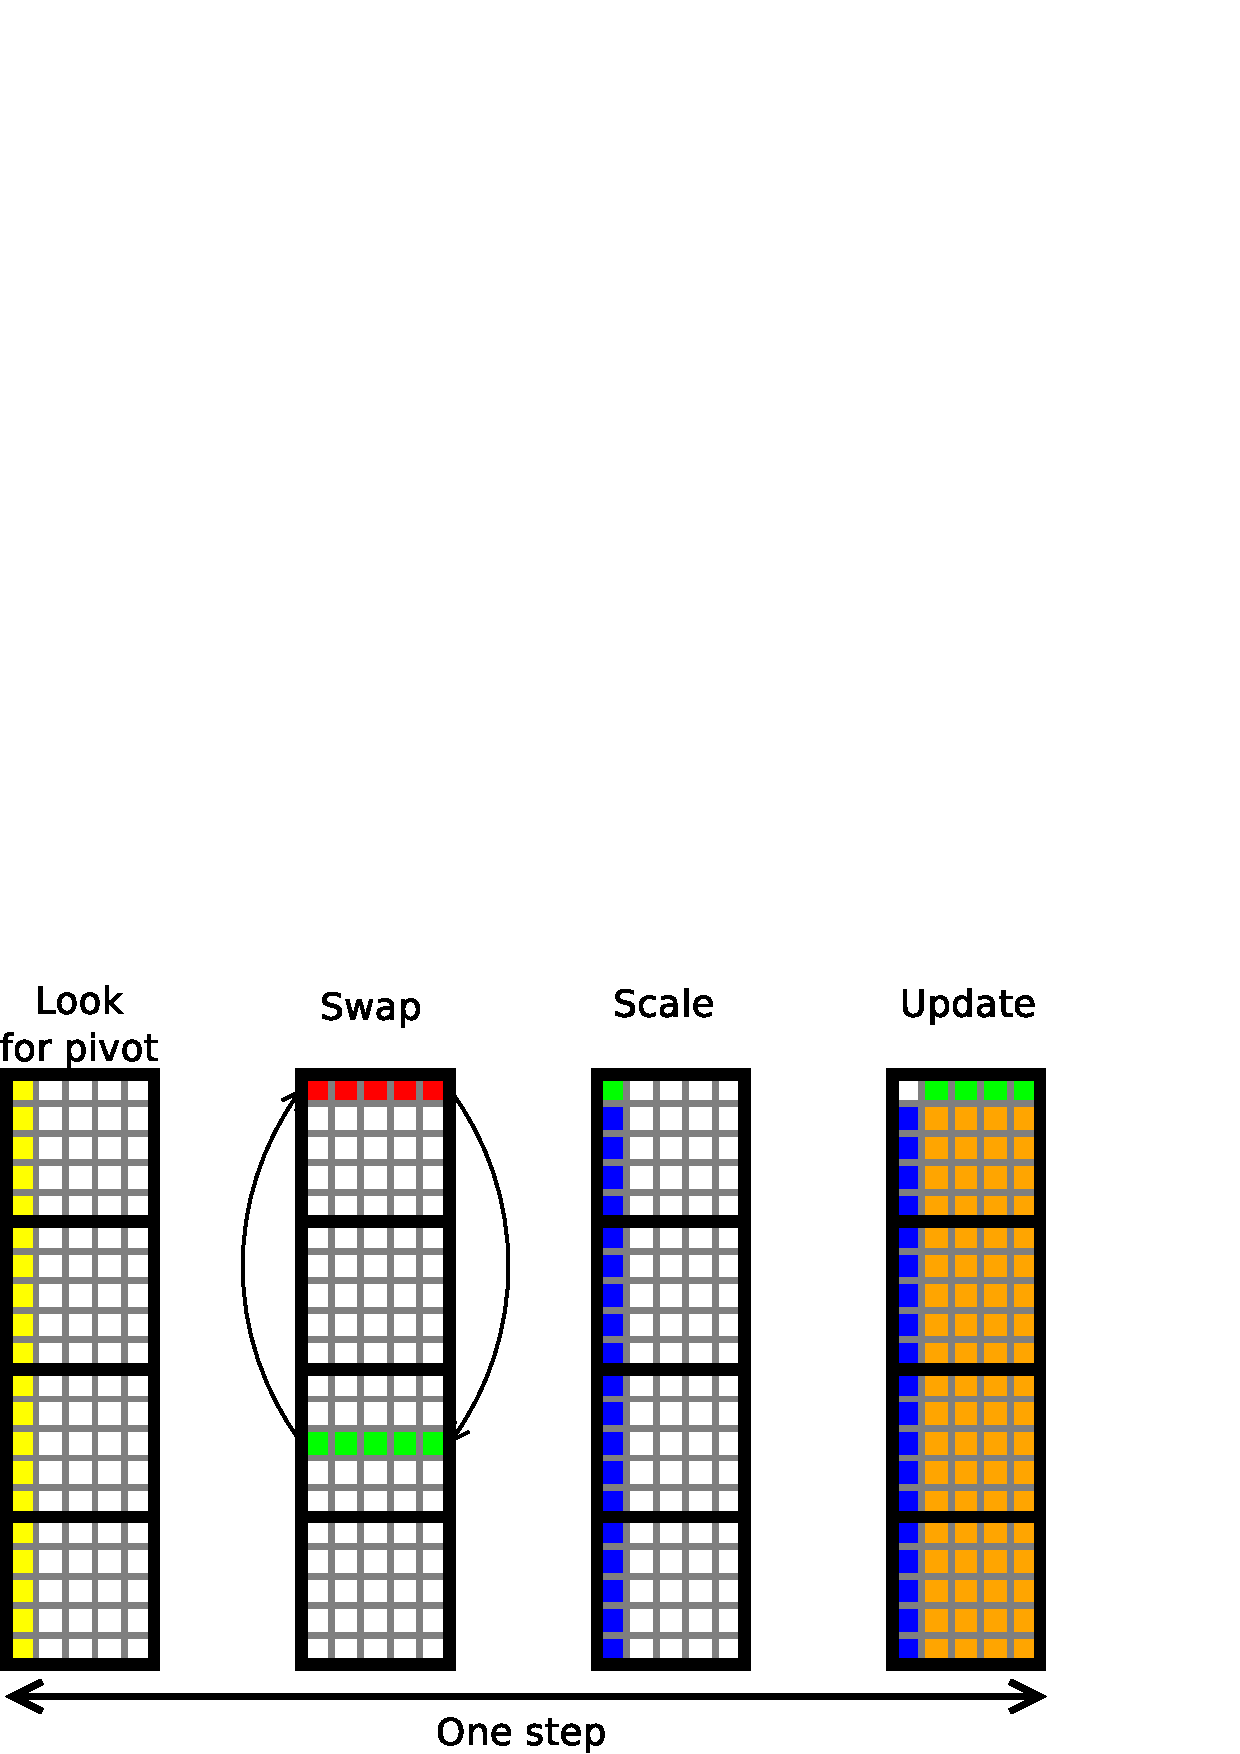
\includegraphics[scale=0.8]{panel_operation.png}
\end{center}
\end{frame}

\begin{frame}{Panel Factorization}
\framesubtitle{Look of maximum}
\begin{columns}
\begin{column}{.30\textwidth}
\begin{center}
\includegraphics[scale=0.8]{panel_max.png}
\end{center}
\end{column}
\hfill
\begin{column}{.70\textwidth}
Each tile sends its maximum row to the main tile.
\begin{center}
\begin{exampleblock}{}
$\Longrightarrow$ Number of communications : $MT*NB$\\
$\Longrightarrow$ Number of tasks : $2*MT$
\end{exampleblock}{}
\end{center}
\end{column}
\end{columns}
\end{frame}

\begin{frame}{Panel Factorization}
\framesubtitle{Swap}
\begin{columns}
\begin{column}{.30\textwidth}
\begin{center}
\includegraphics[scale=0.8]{panel_swap.png}
\end{center}
\end{column}
\hfill
\begin{column}{.70\textwidth}
Each tile need the new swap row.
\begin{center}
\begin{exampleblock}{}
$\Longrightarrow$ Number of communications : $MT*NB$\\
$\Longrightarrow$ Number of tasks : $MT$
\end{exampleblock}{}
\end{center}
\end{column}
\end{columns}
\end{frame}

\begin{frame}{Panel Factorization}
\framesubtitle{Scale and Update}
\begin{columns}
\begin{column}{.25\textwidth}
\begin{center}
\includegraphics[scale=0.8]{panel_scale.png}
\end{center}
\end{column}
\hfill
\begin{column}{.25\textwidth}
\begin{center}
\includegraphics[scale=0.8]{panel_update.png}
\end{center}
\end{column}
\hfill
\begin{column}{.50\textwidth}
The two operations may be executed in the same task.
\begin{center}
\begin{exampleblock}{}
$\Longrightarrow$ the two operations are executed in the same task of the swap
\end{exampleblock}{}
\end{center}
\end{column}
\end{columns}
\end{frame}

\begin{frame}{Panel Factorization}
\framesubtitle{Comparative study}
\begin{itemize}
\item Natural Version
\begin{exampleblock}{}
\begin{itemize}
\item Total tasks : $2 * MT * NB * min(MB,NB)$
\item Total global communications : $2 * MT * min(MB,NB)$
\end{itemize}
\end{exampleblock}{}
\item Implemented Version
\end{itemize}
\end{frame}

\begin{frame}{Panel Factorization}
\framesubtitle{Implemented version}
\begin{columns}
\begin{column}{.70\textwidth}
Optimizations:
\begin{itemize}
\item Look for the maximum locally using thread parallelism
\item Share the local result by using a binary tree
\item Share the global result by using Bruck's algorithm
\item Use internal blocking
\end{itemize}
\end{column}
\hfill
\begin{column}{.30\textwidth}
\end{column}
\end{columns}
\end{frame}

\begin{frame}{Panel Factorization}
\framesubtitle{Implemented version}
\begin{columns}
\begin{column}{.70\textwidth}
Optimizations:
\begin{itemize}
\item Look for the maximum locally using thread parallelism
\transparent{0.4}
\item Share the local result by using a binary three
\item Share the global result by using Bruck's algorithm
\item Use internal blocking
\end{itemize}
\end{column}
\hfill
\begin{column}{.30\textwidth}
\begin{center}
\includegraphics[scale=0.8]{panel_max_opt1.png}
\end{center}
\end{column}
\end{columns}
\pause
\begin{exampleblock}{}
$\Longrightarrow$ Number of tasks : $MT$
\end{exampleblock}{}
\end{frame}

\begin{frame}{Panel Factorization}
\framesubtitle{Implemented version}
\begin{columns}
\begin{column}{.70\textwidth}
Optimizations:
\begin{itemize}
{\transparent{0.4}
\item Look for the maximum locally using thread parallelism}
\item Share the local result by using a binary three
\transparent{0.4}
\item Share the global result by using Bruck's algorithm
\item Use internal blocking
\end{itemize}
\end{column}
\hfill
\begin{column}{.30\textwidth}
\begin{center}
\includegraphics[scale=0.6]{binary_reduction.png}
\end{center}
\end{column}
\end{columns}
\pause
\begin{exampleblock}{}
$\Longrightarrow$ Number of tasks : $MT$\\
$\Longrightarrow$ Number of local communications : $MT/P$
\end{exampleblock}{}
\end{frame}

\begin{frame}{Panel Factorization}
\framesubtitle{Implemented version}
\begin{columns}
\begin{column}{.50\textwidth}
Optimizations:
\begin{itemize}
{\transparent{0.4}
\item Look for the maximum locally using thread parallelism
\item Share the local result by using a binary three}
\item Share the global result by using Bruck's algorithm
\transparent{0.4}
\item Use internal blocking
\end{itemize}
\end{column}
\hfill
\begin{column}{.50\textwidth}
\begin{center}
\includegraphics[scale=0.5]{bruck.png}
\end{center}
\end{column}
\end{columns}
\pause
\begin{exampleblock}{}
$\Longrightarrow$ Number of tasks : $log(P)$\\
$\Longrightarrow$ Number of global communications : $log(P)$
\end{exampleblock}{}
\end{frame}

\begin{frame}{Panel Factorization}
\framesubtitle{Implemented version}
\begin{columns}
\begin{column}{.50\textwidth}
Optimizations:
\begin{itemize}
{\transparent{0.4}
\item Look for the maximum locally using thread parallelism
\item Share the local result by using a binary three
\item Share the global result by using Bruck's algorithm}
\item Use internal blocking
\end{itemize}
\end{column}
\hfill
\begin{column}{.50\textwidth}
\begin{center}
\includegraphics[scale=0.5]{panel_opt2.png}
\end{center}
\end{column}
\end{columns}
\end{frame}

\begin{frame}{Panel Factorization}
\framesubtitle{Comparative study}
\begin{itemize}
\item Natural Version
\begin{exampleblock}{}
\begin{itemize}
\item Total tasks : $2 * MT * NB * min(MB,NB)$
\item Total global communications : $2 * MT * min(MB,NB)$
\end{itemize}
\end{exampleblock}{}
\item Implemented Version
\begin{exampleblock}{}
\begin{itemize}
\item Total tasks : $(2 * MT + log(P)) * min(MB,NB)$
\item Total global communications : $log(P) * min(MB,NB)$
\end{itemize}
\end{exampleblock}{}
\end{itemize}
\end{frame}
